\documentclass[11pt,onecolumn]{article}

% ==========================================================
% NSF SaTC-style project description template
% Notes:
%   - NSF does not provide one fixed SaTC LaTeX template.
%   - This file follows common NSF PAPPG formatting practice:
%     letter paper, single column, 1 inch margins, 11pt font.
%   - Check the current solicitation/PAPPG before submission.
% ==========================================================

\usepackage[letterpaper,margin=1in]{geometry}
\usepackage{times}
\usepackage{graphicx}
\usepackage{wrapfig}
\usepackage{subcaption}
\usepackage{booktabs}
\usepackage{multirow}
\usepackage{array}
\usepackage{enumitem}
\usepackage{xcolor}
\usepackage{soul}
\usepackage{amsmath,amssymb}
\usepackage{url}
\usepackage{xspace}
\usepackage[colorlinks=true,linkcolor=blue,citecolor=blue,urlcolor=blue]{hyperref}
\usepackage{titlesec}
\usepackage{caption}
\usepackage{wrapfig}
\usepackage{comment} 
\usepackage{amsmath}   % Required for proper math formatting and subscript handling
\usepackage{graphicx}  % Required if you are embedding an architecture diagram

% Spacing: avoid overly tight formatting for NSF compliance.
\linespread{1.0}
\setlength{\parindent}{1.5em}
\setlength{\parskip}{0pt}
\setlist[itemize]{leftmargin=1.25em,itemsep=0.12em,topsep=0.15em}
\setlist[enumerate]{leftmargin=1.45em,itemsep=0.12em,topsep=0.15em}
\titlespacing*{\section}{0pt}{0.75em}{0.35em}
\titlespacing*{\subsection}{0pt}{0.60em}{0.25em}
\titlespacing*{\subsubsection}{0pt}{0.45em}{0.15em}
\captionsetup{font=small,labelfont=bf}

\newcommand{\sys}{\textsc{Vest}\xspace}
\newcommand{\byotee}{\textsc{BYOTee}\xspace}
\newcommand{\enola}{\textsc{ENOLA}\xspace}

\newcommand{\etal}{\textit{et al.}}

\newcommand{\arman}[1]{%
	\begingroup
	\definecolor{hlcolor}{RGB}{135, 216, 230}\sethlcolor{hlcolor}%
	\textcolor{black}{\hl{\textit{\textbf{Arman:} #1}}}%
	\endgroup
}

\title{\vspace{-1.2em}\textbf{SaTC 2.0: RES: VEST: Verifiable Trust Establishment on Embedded Systems}\vspace{-1.0em}}
\author{}
\date{}
%\pagestyle{empty}
%\pagenumbering{gobble}
\begin{document}
	\maketitle
	\vspace{-2.0em}
	
% !TEX root = main.tex
% ==========================================================
\section{Overview and Objectives}
\label{sec:overview}
% ==========================================================

Embedded and cyber-physical systems have become fundamental components of modern computing infrastructure, supporting sensing, communication, control,
and decision-making in applications ranging from industrial automation and transportation to medical devices, smart infrastructure, and the Internet of
Things (IoT).
The scale of this infrastructure is already immense and continues to grow: ARM alone has shipped more than 200 billion chips to date, with
Cortex-M microcontrollers which is the class of device this proposal targets~\cite{arm2021chips}.
This accounts for nearly half of that cumulative total and three-quarters of
annual shipments, while the number of connected IoT devices is projected to reach 39 billion by the end of
2030~\cite{iotanalytics2025}.
Unlike traditional desktop and server systems, embedded devices often operate under tight computation, memory, energy, and timing constraints,
interact directly with sensors and actuators, while remaining field deployed for years without any inspection of their software.
Consequently, compromise of an embedded device can affect not only software confidentiality and integrity, but also the physical
processes that the device monitors or controls, and it can remain undetected for as long as no operator is present to notice anomalous behavior.
Recognizing these risks, recent guidance from multiple federal agencies now requires device-level cybersecurity capabilities spanning exactly the application domains named above: NIST's IoT Core Baseline profile underlies the U.S. Cyber Trust Mark consumer-labeling program~\cite{nist2022ir8425}, the FDA's 2023 premarket cybersecurity guidance is now a statutory requirement for medical devices~\cite{fda2023cybersecurity}, and CISA's Secure-by-Design principles, joined by seventeen U.S.\ and international partner agencies, call for the same shift toward built-in, continuously verifiable device trustworthiness this proposal pursues~\cite{cisa2023sbd}.

These risks are not hypothetical.
In July 2025, researchers exploited Bluetooth-stack vulnerabilities to achieve remote code execution on the infotainment ECUs of vehicles from Mercedes-Benz, Volkswagen, and \v{S}koda~\cite{perfektblue2025}.
Beginning in 2023, attackers compromised programmable logic controllers (PLCs) across U.S. water and wastewater utilities using nothing more than default credentials, in one case seizing control of a Pennsylvania utility's booster station~\cite{cisa2023unitronics}.
In 2020, a single vulnerable TCP/IP library embedded in hundreds of millions of devices across the healthcare, industrial, and transportation sectors was shown to allow remote code execution through one crafted network packet~\cite{cisa2020ripple20}, and a separate set of memory-corruption vulnerabilities disclosed the same year affected FreeRTOS+TCP itself~\cite{zimperium2018freertos}.
Each incident shares a common structure: a memory-corruption or authentication flaw in one embedded software component was sufficient to compromise the physical behavior of a field-deployed, unattended device, with only a slow and costly recall or firmware push as remedy.
\textbf{Because embedded and cyber-physical devices cannot rely on a human to notice compromise or a routine patch cycle to fix it, establishing and continuously verifying their trustworthiness, remotely and throughout deployment, is essential, not merely desirable.}

The firmware and software of these systems are commonly developed in memory-unsafe languages such as C and C++, and most resource-constrained MCUs
provide weak process isolation due to the absence of a memory management unit (MMU), and hardware privilege is limited to only two levels: privileged and unprivileged, rather than a ring or exception-level hierarchy.
As a result, the memory-corruption vulnerabilities above routinely lead to control-flow hijacking, unauthorized memory or peripheral access, and complete software compromise.
Modern embedded platforms increasingly provide improved hardware security mechanisms, including secure boot, memory protection units (MPUs), trusted
execution environments (TEEs), hardware cryptographic engines, and architectural control-flow protection such as ARM's Pointer Authentication and
Branch Target Identification extension~\cite{m85}.
However, the presence of these mechanisms alone neither guarantees that the hardware/software composition of the system can be verified nor that its
trustworthiness holds throughout later execution.

\textbf{First, existing systems provide limited ability to determine precisely what constitutes the trusted execution environment.}
TEEs isolate security-sensitive software from less-trusted software and have become an important foundation for embedded security.
However, conventional TEE designs typically expose a fixed, platform-defined trusted computing base (TCB). Trusted and untrusted workloads may share processors, caches, memory hierarchies, interrupt infrastructure, and peripherals, while applications are given limited ability to select the hardware and software resources that should belong to their trusted environment. As a result, the trusted boundary may contain resources and privileged software that are unnecessary for a particular
application, increasing both the TCB and the potential attack surface.
Reconfigurable embedded hardware provides an opportunity to rethink this assumption: FPGA-based SoCs can construct isolated execution domains using explicitly selected processing, memory, peripheral, and communication resources~\cite{armanuzzaman2024building}. Yet a fundamental question remains: \emph{how can an embedded system construct an application-specific trusted execution environment whose hardware and software composition can itself be verified by a remote party?}

\textbf{Second, establishing a trusted environment does not guarantee that its software continues to execute as intended.}
Secure boot and conventional remote attestation can establish properties of software identity or initial system state, but a correctly loaded program can later be compromised through a runtime vulnerability. Control-flow attestation (CFA) addresses this gap by allowing a remote verifier to reason about the execution path taken by a program~\cite{abera2016c,dessouky2017fat,sun2020oat,yadav2023whole}. However, existing CFA approaches remain difficult to apply to resource-constrained and long-running embedded workloads. Evidence may grow with execution duration or program complexity, while software-based measurement, protected-domain transitions, and cryptographic operations can introduce significant runtime overhead.
Moreover, realistic embedded systems are event driven: interrupts, exception handling, callbacks, RTOS scheduling, task transitions, and context switches can alter execution in ways that are not adequately represented by a simple single-program control-flow trace.
Thus, a second fundamental question is: \emph{how can embedded systems provide scalable and protected runtime evidence that enables a verifier to reason about authorized execution across bare-metal and multitasking environments without evidence growing with execution duration?}

\textbf{Third, existing trusted execution mechanisms provide limited support for preserving trust after a localized compromise.}
A TEE is often treated as a single trusted domain even though it may contain multiple components, such as application logic, cryptographic services, parsers, communication code, and peripheral drivers. A vulnerability in one such component can therefore expose resources belonging to the entire trusted domain. Fine-grained compartmentalization can reduce this blast radius by restricting each component to the code, data, and peripherals that it requires.
On resource-constrained MCUs, however, compartmentalization introduces additional challenges because MPU regions are limited and protection-state changes frequently require privileged transitions and reconfiguration.
Furthermore, combining spatial isolation with architectural control-flow protection is not straightforward: shared authentication state, common runtime code, asynchronous interrupts, and partially updated protection state can create new cross-compartment attack opportunities.
Even where isolation and control-flow protection are both correctly enforced, existing systems constrain how compartments may communicate but not what they may do with the data they legitimately exchange, leaving a confused-deputy vulnerability that no control-flow policy can detect.
Existing mechanisms also provide little information to a remote verifier about which trusted component was affected by a violation and whether unaffected components can safely continue operation.

These limitations reveal a broader scientific gap: \textbf{embedded trust is typically treated as a property established at a particular point in time, rather than as a property that must be established, verified, and preserved throughout system execution.}
Knowing that the expected software was loaded does not establish whether the execution environment contained only the necessary trusted resources; knowing the initial environment does not establish whether the software subsequently followed authorized behavior; and detecting a runtime violation does not by itself determine which part of the trusted system must lose trust. Addressing these questions independently therefore leaves gaps between trusted-environment construction, runtime verification, and post-compromise response.

This project proposes \textbf{VEST: Verifiable Trust Establishment for Embedded Systems}, with the objective of developing a continuous trust model for
resource-constrained embedded systems. VEST will investigate how trusted execution environments can be constructed from explicitly selected hardware and
software resources and exposed to a remote verifier; how hardware-assisted runtime evidence can efficiently represent control-flow, task, interrupt, and
other security-relevant execution events; and how runtime evidence can be combined with fine-grained isolation to determine the scope of a violation,
contain affected components, and selectively restore and re-attest them.
Rather than treating trusted execution, runtime attestation, and compartmentalization as independent mechanisms, \sys will connect them through a common trust lifecycle in which the verifier can reason about \emph{what environment was established}, \emph{how that environment executed}, and \emph{what remains trustworthy following a localized compromise}.

Accordingly, the project is driven by three overarching research objectives:

\begin{itemize}
	\item \textbf{O1: Establish verifiable application-specific trust.}
	Develop architectures and resource-composition mechanisms that construct
	trusted execution environments according to application requirements and
	enable remote verification of their security-relevant hardware and software
	configuration.
	
	\item \textbf{O2: Maintain trust through scalable runtime evidence.}
	Develop efficient runtime measurement and verification techniques for
	bare-metal and RTOS-based embedded systems that capture security-relevant
	execution while bounding measurement and communication overhead.
	
	\item \textbf{O3: Preserve trust after localized compromise.}
	Develop evidence-guided compartmentalization, containment, recovery, and
	re-attestation mechanisms that identify affected trusted domains while
	allowing confidence in unaffected components to be retained.
\end{itemize}

Achieving these objectives will move embedded-system security beyond
one-time trust establishment toward a model in which trust can be continuously
reasoned about from system construction, through runtime execution, to
containment and recovery following compromise.
\begin{figure}[t]
	\centering
	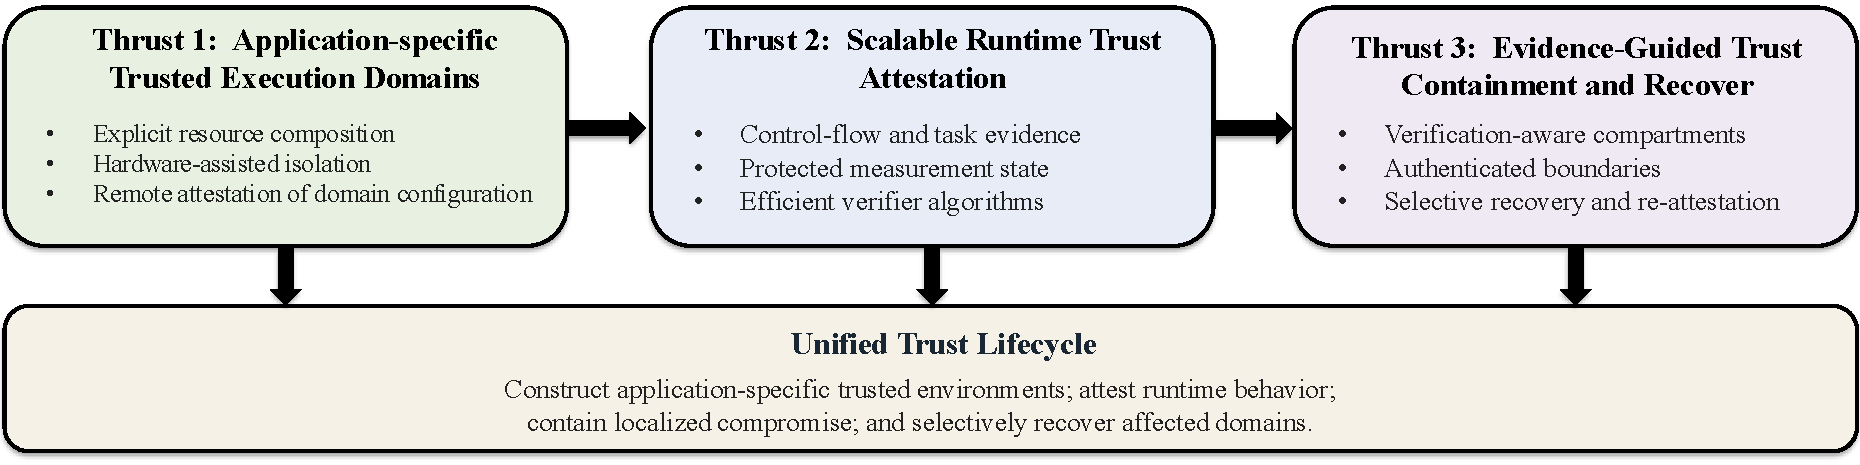
\includegraphics[width=0.98\linewidth]{figs/VEST_thrusts.pdf}
	\caption{Proposed research trusts of \sys}
	\label{fig:thrusts}
\end{figure}

\subsection{Proposed Research}
As illustrated in Figure~\ref{fig:thrusts}, this proposal presents a comprehensive three-step research agenda, namely \sys: \textit{\underline{V}erifiable Trust \underline{E}stablishment for Embedded \underline{S}ys\underline{t}ems}, driven by the following overarching scientific goal:
Designing and developing novel system architectures, algorithms, and compiler techniques that establish \textbf{application-specific trusted execution environments}, \textbf{continuously verify their runtime behavior}, and preserve trust through \textbf{localized containment and recovery}.

To establish trust, \sys will construct application-specific trusted execution domains whose processing, memory, peripheral, communication, acceleration, and attestation resources are explicitly selected and remotely verifiable.
To maintain trust, \sys will develop scalable runtime attestation for bare-metal and RTOS-based systems, with evidence that captures control flow, task transitions, interrupts, and other security-relevant events without growing with execution duration.
To preserve trust after compromise, \sys will combine runtime evidence with verification-aware compartmentalization to localize violations, enforce authenticated boundaries, and selectively recover and re-attest affected domains while retaining trust in unaffected components.

We plan to realize this vision by leveraging embedded-system-specific hardware capabilities—including configurable processing resources, memory protection, trusted execution support, hardware cryptographic engines, and control-flow protection—through the following three research thrusts:

\textbf{Thrust 1: Application-Specific Trusted Execution Domains.}
Conventional embedded TEEs multiplex trusted and untrusted workloads on the same processor and rely on fixed, platform-defined trust boundaries. Sharing processor time, caches, memory hierarchies, interrupt logic, and peripherals can introduce temporal interference, increase cross-domain exposure, and create side-channel risks. Moreover, applications cannot tailor the trusted hardware and software resources to their security requirements.

This thrust will develop methods for constructing application-specific trusted execution domains from explicitly selected processing, memory, peripheral, communication, acceleration, and attestation resources. We will investigate new system architectures, resource-allocation and composition algorithms, hardware-assisted isolation, and attestation protocols that expose the security-relevant domain configuration to a remote verifier. The resulting domains will allow a verifier to confirm both the trusted software and the execution environment that protects it.

\textbf{Thrust 2: Scalable Runtime Trust Attestation.}
Control-flow attestation enables a remote verifier to determine whether embedded software followed an authorized execution path and thereby detect control-flow hijacking. However, existing approaches are difficult to deploy on resource-constrained and long-running systems because their evidence can grow with program complexity or execution duration. Measurement computation, trusted-world transitions, and protection of cryptographic state can also impose substantial overhead, while support for interrupts, asynchronous events, and multitasking execution remains limited.

This thrust will develop scalable runtime trust attestation for both bare-metal and RTOS-based systems. Control-flow evidence will form the core of the attestation and will be augmented with task transitions, context switches, interrupt execution, and selected security-critical interactions. We will develop novel evidence-compression and verification algorithms, compiler-based instrumentation, protected measurement runtimes, and hardware-assisted cryptographic mechanisms. The proposed methods will bound evidence size by static program and task structure rather than execution duration while enabling efficient remote verification.

\textbf{Thrust 3: Evidence-Guided Trust Containment and Recovery.}
Existing MCU compartmentalization mechanisms isolate code, data, and peripherals using the MPU, but frequent privileged transitions and MPU reconfiguration can impose substantial switching overhead, and none analyzes correctness under nested, preempting interrupts. Moreover, naively composing spatial isolation with control-flow protection introduces new cross-domain risks: shared authentication keys may permit signed control-flow state to be reused across compartments, shared runtime code can enlarge the valid branch-target set, and interrupts or faults may execute outside the active sandbox or observe partially updated protection state. Even where isolation and control-flow protection are both enforced, existing systems constrain how compartments may communicate but not what they may do with the data they legitimately exchange -- a confused-deputy gap that lets a compromised compartment corrupt a co-resident compartment's state without ever violating a control-flow policy. Existing approaches also provide limited support for identifying the affected domain and preserving trust in unaffected components after a violation.

This thrust will develop real-time- and data-flow-aware compartmentalization with interrupt-safe transitions. We will design compiler-driven partitioning algorithms that jointly reason about MPU region constraints, real-time budgets, and DMA-capable peripherals; a formally verified transition monitor that routes every cross-compartment transfer through a fixed-priority exception rather than ad hoc interrupt masking; ambiguity-guided data-flow policies that enforce directional (read/write) MPU permissions where a dependence analysis can resolve a shared location's legitimate writer, and fall back to hardware-authenticated write tags only where it cannot; and evidence-guided recovery protocols that localize a violation to the affected compartment, contain it, and selectively restore and re-attest the rest of the system.

\textbf{Intellectual Merit.}
This project will advance the system architectures, hardware/software TCB design, and algorithms needed to establish, verify, and preserve trust in embedded systems.
It will develop application-specific trusted execution domains with verifiable resource composition and isolation; scalable runtime attestation for bare-metal and RTOS-based systems; and evidence-guided compartmentalization for localized containment, recovery, and re-attestation. 
Together, these contributions will create a continuous trust lifecycle spanning trusted-environment construction, runtime verification, and post-compromise restoration.

\subsection{Relevance to SaTC}

\subsection{PI Qualifications}

% !TEX root = main.tex
\section{Background}
\textbf{Architecture.}
This project targets three representative embedded platform classes: FPGA SoCs, which couple a fixed processor subsystem with reconfigurable programmable logic; ARM Cortex-A systems implementing Armv9.2-A's Realm Management Extension (RME) of the ARM Confidential Compute Architecture (CCA); and ARM Cortex-M microcontrollers (MCUs).
The FPGA's processor subsystem runs system software and manages external memory, while its programmable logic can be configured into soft-core processors, peripherals, and custom interconnects.
Cortex-A processors run Linux-class software under an MMU-based exception-level hierarchy.
Armv9.2-A's optional RME extends TrustZone's Normal and Secure worlds with a Realm and a Root world, whose EL3 monitor programs the Granule Protection Table (GPT) to assign each physical granule to a world, enforced in hardware by the Granule Protection Check (GPC).
Cortex-M MCUs run bare-metal firmware or lightweight RTOS workloads with only privileged and unprivileged execution states, and recent architectures add security features such as TrustZone, memory protection units (MPUs), and hardware cryptographic support.

\textbf{Trusted Execution Environments.}
Trusted execution environments (TEEs) use hardware-enforced isolation to separate a trusted domain, which may host cryptographic services and secure storage, from an untrusted domain running the remaining firmware or OS software, with controlled interfaces governing communication across the boundary.
On Cortex-A, TrustZone's Normal and Secure worlds are separated by an EL3 monitor reached via the \texttt{SMC} instruction, further partitioned by RME as described above.
On Cortex-M, TrustZone enforces separation through controlled transitions -- designated entry points, security-aware control-transfer instructions (i.e., \texttt{SG}, \texttt{BLNS}), and protected exception handling.
FPGA SoCs may add hard-core Cortex-A or RISC-V TEE support, or construct additional domains from soft-core logic.
A TEE's security ultimately depends on the correctness of its trusted software and the integrity of the hardware that enforces the isolation boundary.

\textbf{Hardware-Assisted Isolation and Cryptography.}
Beyond software-configurable isolation, both processor classes used in this project expose dedicated hardware for security enforcement.
On Cortex-A, the GPC checks every physical access against the Root-world monitor's GPT in hardware, so RME's world isolation holds at the granularity of individual memory granules even if the OS or hypervisor above the monitor is compromised~\cite{li2022design,armcca}.
On Cortex-M, the ARM Cortex-M85 implements the ARMv8.1-M Pointer Authentication (PA) extension, which uses the QARMA tweakable block cipher to generate keyed Pointer Authentication Codes (PACs) over pointer or data values via instructions such as \texttt{PAC} and \texttt{PACG}, with keys drawn from dedicated, non-memory-mapped 128-bit registers selected by security state and privilege level~\cite{m85,avanzi2017qarma}.
Hardware-assisted PA computation is substantially faster than software-based cryptographic measurement: on a 25 MHz Cortex-M85, a single \texttt{PACG} operation requires approximately 12 CPU cycles, versus 5,768 cycles for an optimized software BLAKE2s computation, at least a \textbf{480$\times$ speedup}.

% !TEX root = main.tex
\section{System and Threat Model}
\label{sec:system_threat}

We consider embedded systems based on FPGA SoC platforms, ARM Cortex-A processors with Armv9.2-A RME, and ARM Cortex-M microcontroller units (MCUs).
FPGA SoCs provide programmable logic composed of configurable logic blocks, Adaptive Logic Modules (ALMs), lookup tables (LUTs), flip-flops, etc. resources that can be interconnected to construct customized hardware modules or soft-core CPUs.
Cortex-A CCA platforms, we treat the Normal world and all Secure-world software, including the TEE OS, partition manager, and drivers, as untrusted, and trust only the Root-world monitor and the RME hardware.
On Cortex-M MCU systems execute bare-metal firmware or an RTOS with multiple tasks, interrupt handlers, and peripheral-facing components.
We assume the availability of hardware security mechanisms such as secure boot, a TEE, memory protection, and hardware support.
A remote verifier is assumed to maintain the expected hardware/software configuration and verify evidence generated by the embedded device.

Our threat model evolves with the \sys~trust lifecycle.
In the first thrust, during trust establishment, an adversary may attempt to cause an unauthorized hardware or software configuration to be accepted as trusted, for example by leaving a peripheral, interrupt, or DMA master outside the attested domain boundary while still presenting the domain as fully isolated.
In the second thrust, during runtime execution, the adversary may exploit memory-corruption vulnerabilities in applications, libraries, drivers, RTOS components, or interrupt handlers (e.g., ROP, JOP, or data-only attacks) to hijack control flow, corrupt measurement state, or interfere with attestation through interrupts and task transitions.
In the third thrust, a compromised component may attempt to cross compartment boundaries, replay authenticated state, or access unauthorized memory and peripherals, for example through non-control-data/confused-deputy attacks that corrupt shared state without violating control-flow policy or by manipulating CPU-writable DMA descriptor fields to redirect a transfer.
We assume that the root of trust and immutable trusted components are correctly provisioned, secure hardware primitives, and protected key registers cannot be modified by unauthorized software.
Physical invasive attacks and destructive denial-of-service attacks are outside the scope.

% !TEX root = main.tex
\section{Research Thrusts}
The scientific contributions of this work is to enable verifiable trust establishment of embedded sysetms by designing and developing novel system architectures, algorithms, and compiler techniques.


% !TEX root = main.tex
\subsection{Thrust 1: Application-Specific Trusted Execution Domains.}
\label{sb:t1}

\textbf{Problem Statement.}
Trusted execution environments (TEEs) provide an important foundation for protecting security-sensitive computation, but their trust boundaries are typically determined by the underlying platform rather than by the requirements of individual applications~\cite{mccune2008flicker,hua2017vtz,koeberl2014trustlite,brasser2019sanctuary,sun2015trustice}.
Different embedded applications, however, have fundamentally different security and resource requirements. One application may require only a processor, private memory, and access to a sensor, while another may additionally require communication interfaces, cryptographic services, or other peripherals~\cite{armanuzzaman2024building,hwang2021ambassy,teeod}.
Nevertheless, conventional TEEs often expose these applications to a fixed hardware/software trusted computing base (TCB), causing them to trust resources and privileged components that are unnecessary for their execution~\cite{schneider2020pie,gross2019breaking,cerdeira2020sok}.
This over-provisioning violates least privilege, enlarges the TCB, and increases the attack surface; in ARM TrustZone, for instance, privileged Secure-world software shares one hardware protection domain and can read all Normal-world memory~\cite{pinto2019demystifying,cerdeira2022rezone,kuhne2024aster}.

A second limitation is that the composition of the trusted environment is often not explicit to a remote verifier~\cite{lebedev2019sanctorum,nunes2019vrased,armanuzzaman2024building}.
Existing attestation mechanisms primarily establish the identity or integrity of trusted software, while the verifier must largely assume that the underlying processors, memory, peripherals, communication paths, and protection mechanisms constitute the intended execution environment~\cite{nunes2019vrased,armanuzzaman2024building}.
Consequently, verifying that the expected software was loaded does not necessarily establish that it executes within the intended hardware/software trust boundary.
The challenge is therefore not only to isolate trusted software, but also to make the resources that constitute its trusted execution environment \emph{application-specific, explicit, and verifiable}.

This thrust asks the following fundamental question: \textbf{\textit{How can embedded systems construct application-specific trusted execution domains from explicitly selected hardware and software resources, while allowing a remote verifier to establish that the intended trust boundary has actually been instantiated?}} Addressing this question requires new abstractions and mechanisms for resource specification and composition, hardware-assisted isolation, and remote attestation of the resulting domain configuration. The resulting trusted execution abstraction should be applicable across embedded architectures that provide suitable isolation and configurable resource mechanisms, rather than being tied to a particular hardware platform.


\textbf{Related Work.}
Prior work has explored more flexible trusted execution along several lines, but none makes the composition of an application-specific trusted domain remotely verifiable on off-the-shelf hardware. vTZ~\cite{hua2017vtz}, Sanctuary~\cite{brasser2019sanctuary}, TrustICE~\cite{sun2015trustice}, uTango~\cite{oliveira2021utango}, and Keystone~\cite{Keystone2020} construct multiple isolated domains by virtualizing TrustZone, partitioning memory access, running a normal-world monitor, using Cortex-M's secure attribution unit, or configuring RISC-V's PMP, respectively, but in each case the TEE and REE still time-share the same CPU and other hardware resources, leaving them susceptible to side-channel attacks rather than truly separated~\cite{armanuzzaman2024building}. CURE~\cite{bahmani2021cure}, Composite Enclaves~\cite{schneider2020pie}, and HECTOR-V~\cite{nasahl2020hector} instead grant exclusive access to specific resources -- cores, caches, or peripherals -- but all three depend on RISC-V's PMP feature or custom hardware extensions unavailable on deployed, off-the-shelf platforms. SGXIO~\cite{weiser2017sgxio} and SGX-FPGA~\cite{xia2021sgx} instead focus narrowly on protecting the I/O path between a CPU and an accelerator, rather than the composition of a trusted domain as a whole. On ARM, ReZone~\cite{cerdeira2022rezone} reduces TEE privilege by partitioning the TrustZone Secure world into zones, but relies on SoC-specific protection controllers and does not make the zone composition verifiable. Recent CCA work isolates Normal-world user-space applications (Shelter~\cite{zhang2023shelter}), relocates Android TEE services into RMM-managed Realm sandboxes with virtio-based I/O (Aster~\cite{kuhne2024aster}), or attests communication among Realms in cloud settings (Mica~\cite{sadi2026sharing}, CAEC~\cite{abdollahi2026caec}); none applies this to the Secure world or covers the platform resources (MMIO peripherals, interrupts, and DMA masters) that constitute a domain. None of these approaches makes an application's complete hardware/software trust boundary explicit, application-specific, and remotely verifiable as a single checkable property. Thrust~1 addresses this gap by treating trusted-domain composition itself as a verifiable system property.


\begin{comment}

\begin{figure}[!t]
	\centering
	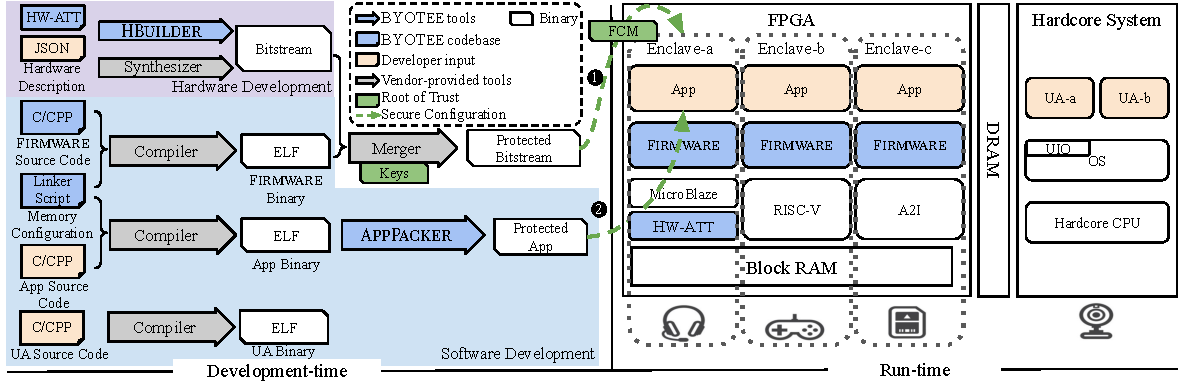
\includegraphics[width=0.98\linewidth]{figs/BYOTee-proposal.pdf}
	\caption{Preliminary foundation of \textit{Thrust 1}: \byotee{} architecture and workflow. The framework creates multiple FPGA-based hardware-software verifiable enclaves with customized  resources, firmware, and peripheral bindings.}
	\label{fig:byotee}
\end{figure}

\end{comment}

\textbf{Task 1.1: Application-Specific Trusted-Domain Composition.}
We will investigate how the security and resource requirements of an embedded application can be translated into an explicit and minimal trusted execution domain. The domain specification will identify the processing, memory, peripheral, communication, acceleration, trusted-software, and attestation resources required by the application, together with the isolation relationships among these resources. We will develop mechanisms for constructing such domains while excluding unnecessary components, unintended communication paths, and privileges that unnecessarily enlarge the trusted computing base.

\begin{wrapfigure}{r}{0.48\textwidth}
	\centering
	\vspace{-8pt}
	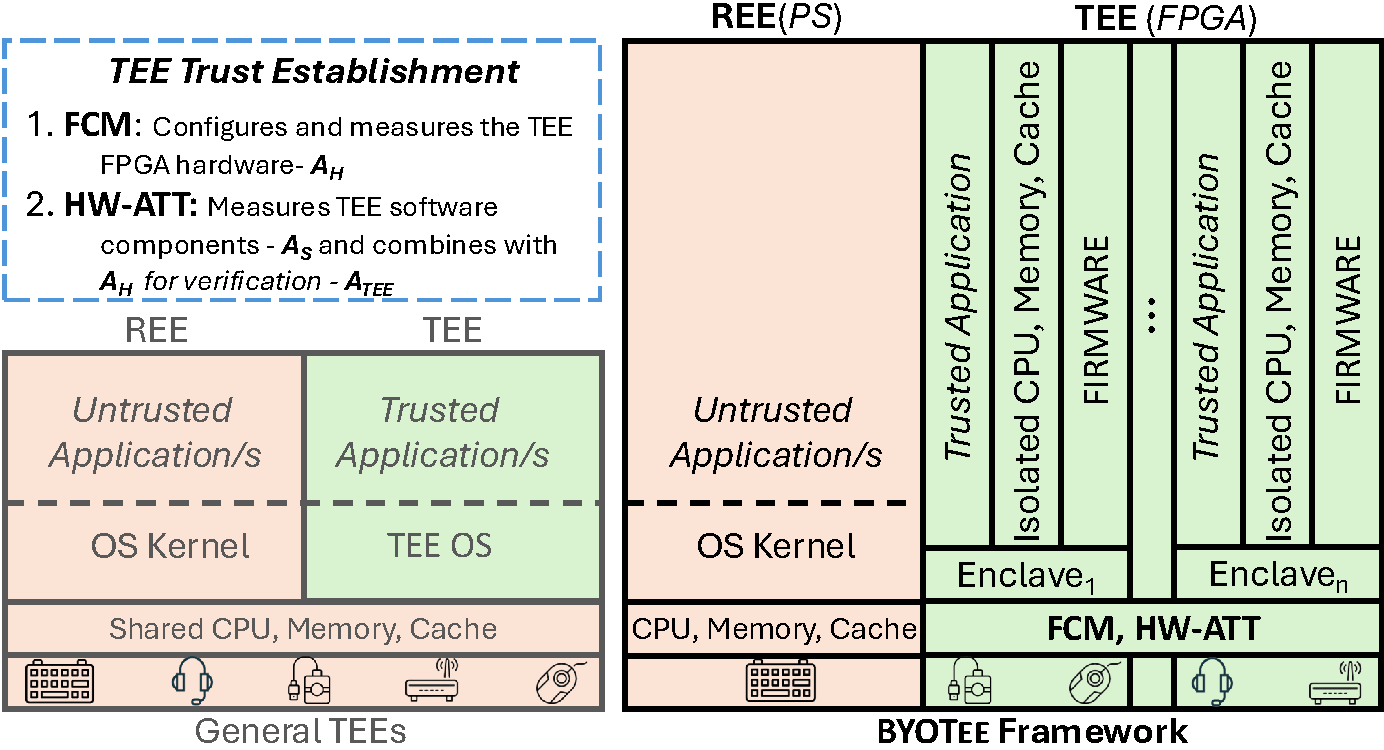
\includegraphics[width=0.48\textwidth]{figs/byotee-overview.pdf}
	\caption{Preliminary foundation of \textit{Thrust 1}: \byotee{} framework enables FPGA-based hardware-software verifiable enclave construction with resource separation.}
	\label{fig:byotee}
	\vspace{-10pt}
\end{wrapfigure}

In our preliminary work, we demonstrated this concept in \byotee~\cite{armanuzzaman2024building} on SoC FPGAs~\cite{FPGA2019}.
As illustrated in Figure~\ref{fig:byotee}, conventional TEEs typically place trusted applications within a common platform-defined boundary in which processor, memory, cache, peripherals, and privileged software may be shared across workloads.
In contrast, \byotee constructs application-specific FPGA enclaves whose hardware and software composition is determined by the requirements of each trusted application.
For each enclave, the developer specifies the required processor configuration, private memory, communication regions, peripherals, and attestation support.
\byotee then allocates and connects only the selected resources, assigns enclave-local address spaces, and generates the corresponding FPGA configuration.
Consequently, each enclave can execute with its own processor, memory, firmware, and application-required peripherals, while FPGA routing isolates these resources and communication paths from the host and other enclaves.
The software TCB is similarly minimized by including only the runtime support, hardware-abstraction components, drivers, and loader required by the protected application.

In addition to constructing the enclave, \byotee introduces two trusted hardware components for establishing the enclave configuration to a remote verifier: the FPGA Configuration Module (\textbf{FCM}) and the hardware attestation module (\textbf{HW-ATT}).
The FCM securely configures and measures the FPGA hardware realization of the trusted enclave, while HW-ATT measures the enclave software and combines the software and hardware measurements into authenticated evidence for remote verification.
Task~1.2 builds on these mechanisms to investigate verifiable trusted-domain establishment across broader embedded architectures.


\begin{wrapfigure}{r}{0.48\textwidth}
	\centering
	\vspace{-8pt}
	\begin{tikzpicture}[
			font=\tiny,
			world/.style={draw, rounded corners=2pt, align=center, inner sep=2pt, text width=1.55cm, minimum height=1.9cm},
			dom/.style={world, fill=green!14},
			arr/.style={-{Latex[length=1.3mm]}, thick},
			darr/.style={{Latex[length=1.3mm]}-{Latex[length=1.3mm]}, thick, dashed},
		]
		% ---- Normal world and decoupled Secure-world domains ----
		\node[world, fill=gray!18] (nw) at (0.8,0) {\textbf{Normal world}\\[2pt] Untrusted OS /\\ hypervisor\\[2pt] \emph{no access to\\ domain memory}\\[2pt] \textbf{Realm world:}\\ RMM unchanged};
		\node[dom] (d1) at (2.9,0)  {\textbf{Domain $D_1$}\\[2pt] SW: TA + libOS\\ Cores: $c_1$\\ Mem: $G_1$\\ MMIO: sensor\\ IRQ: 33 \\ DMA: --};
		\node[dom] (d2) at (4.65,0) {\textbf{Domain $D_2$}\\[2pt] SW: TA + libOS\\ Cores: $c_2$\\ Mem: $G_2$\\ MMIO: crypto\\ IRQ: 45 \\ DMA: $s_1$};
		\node[dom] (d3) at (6.4,0)  {\textbf{Domain $D_3$}\\[2pt] SW: TA + libOS\\ Cores: $c_3$\\ Mem: $G_3$\\ MMIO: NIC\\ IRQ: 52 \\ DMA: $s_2$};
		\draw[darr] ([yshift=3mm]nw.east) -- ([yshift=3mm]d1.west);
		\begin{scope}[on background layer]
			\node[draw, dashed, rounded corners=3pt, fill=green!5, fit=(d1)(d2)(d3), inner sep=2.5pt] (sw) {};
		\end{scope}
		\node[anchor=south, yshift=-1pt] at (sw.north) {\emph{Decoupled Secure world: least-privilege, mutually isolated domains}};

		% ---- Hardware enforcement ----
		\node[draw, rounded corners=2pt, fill=blue!10, align=center, text width=6.9cm, minimum height=0.55cm, inner sep=2pt] (gpc) at (3.6,-1.95)
			{\textbf{Hardware enforcement:} per-core GPC checks every physical access against the core's active GPT view; the SMMU checks DMA against one system-wide GPT};
		\foreach \n/\l in {nw/{V_N}, d1/{V_1}, d2/{V_2}, d3/{V_3}} {
			\draw[arr] ([yshift=-1.5pt]\n.south) -- (\n.south |- gpc.north) node[pos=0.72, right, inner sep=1.5pt] {$\l$};
		}

		% ---- Root monitor and verifier ----
		\node[draw, rounded corners=2pt, fill=yellow!22, align=left, text width=4.5cm, inner sep=3pt] (root) at (2.33,-3.7)
			{\centering\textbf{Root monitor (EL3)}\par\vspace{1pt}
			\raggedright 1.~\textbf{Build:} manifest $M \rightarrow$ disjoint GPT views $V_i$; configure MMIO, SMMU, GIC\\
			2.~\textbf{Switch:} install $V_i$ on the core (SMC); invalidate cached GPT info\\
			3.~\textbf{Measure:} $\mathbf{A}_H$ over $M$, $V_i$, MMIO, SMMU, GIC; $\mathbf{A}_S$ over domain software\par};
		\draw[arr] (root.north) -- (root.north |- gpc.south) node[midway, left, inner sep=1.5pt] {program};
		\node[draw, rounded corners=2pt, fill=violet!10, align=center, text width=1.4cm, inner sep=3pt, minimum height=1.5cm] (ver) at (6.5,-3.7)
			{\textbf{Remote verifier}\\[2pt] checks $\mathbf{A}_{TEE}$ against $M$};
		\draw[arr] ([yshift=2.5mm]ver.west) -- ([yshift=2.5mm]root.east) node[midway, above, inner sep=1pt] {nonce};
		\draw[arr] ([yshift=-2.5mm]root.east) -- ([yshift=-2.5mm]ver.west) node[midway, below, inner sep=1pt] {$\mathbf{A}_{TEE}$};
	\end{tikzpicture}
	\caption{Decoupled Secure world on ARM CCA. The Root monitor turns a domain manifest $M$ into per-domain GPT views enforced by hardware GPC and measures the realized composition as $\mathbf{A}_H$ for $\mathbf{A}_{TEE}$. Dashed arrow: declared shared window.}
	\label{fig:cca}
	\vspace{-10pt}
\end{wrapfigure}

We will extend this composition model to fixed-silicon platforms without custom or reconfigurable hardware, focusing on the Secure world of ARM CCA~\cite{li2022design}.
Today's Secure world is one hardware protection domain: the TEE OS or S-EL2 partition manager, trusted applications, secure drivers, and peripherals share the Secure physical address space, are separated only by fully trusted software, and can read all Normal-world memory.
We will develop a \emph{decoupled Secure world} in which a small Root-world monitor uses the Granule Protection Tables (GPT), which assign each physical granule to a world, and the hardware Granule Protection Check (GPC) to split it into mutually isolated, least-privilege domains, each specified by its cores, memory, MMIO peripherals, DMA masters, interrupts, and explicit channels (Figure~\ref{fig:cca}).
Because a GPT distinguishes only worlds, the monitor installs a separate GPT view on a domain's cores at each domain switch, invalidating cached GPT information; in this view only the domain's own granules and declared shared windows are accessible, so a compromised TEE OS or partition manager reaches neither other domains nor the Normal world.
Since the GPC vets physical addresses after translation, the design needs only new Root-monitor firmware on RME-capable processors and leaves the RMM, realm translation tables, and each domain's page tables untouched. It thus complements \byotee's hardware-level construction with a software-defined one on standard ARM silicon, while the domain specification remains architecture-independent.
The central challenges are (i) exclusively assigning peripherals, interrupts, and DMA masters, which the GPC alone cannot enforce (the SMMU checks DMA against one system-wide GPT and interrupts lie outside the GPT) and which prior CCA work addresses only for user-space applications and Realm VMs~\cite{zhang2023shelter,bertschi2024devlore}, (ii) preserving real-time behavior despite GPT invalidation on every domain switch, and (iii) determining whether a requested domain can be faithfully realized given residual shared state such as caches.



\begin{wrapfigure}{r}{0.48\textwidth}
	\centering
	%	\vspace{-8pt}
	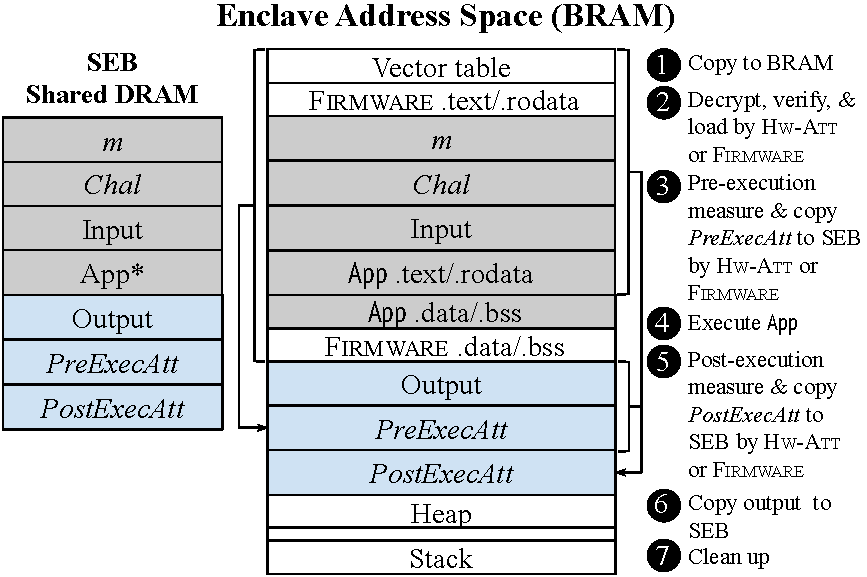
\includegraphics[width=0.46\textwidth]{figs/BYOTee-attestation-proposal.pdf}
	\caption{Verifiable trusted-domain establishment- $\mathbf{A}_{TEE}$. The FPGA Configuration Module (\textbf{\textit{FCM}}) establishes the hardware configuration measurement-  $\mathbf{A}_H$, while \textbf{\textit{HW-ATT}} measures the protected firmware- $\mathbf{A}_S$ and application for remote verification.}
	\label{fig:byotee_attestation}
	\vspace{-10pt}
\end{wrapfigure}

\textbf{Task 1.2: Verifiable Trusted-Domain Establishment.}
We will investigate how a remote verifier can establish that the trusted domain defined in Task~1.1 has actually been instantiated as intended.
Rather than attesting only the protected application, we will bind evidence about the trusted software to measurements of the security-relevant execution environment.
This will allow the verifier to determine whether both the hardware and software components of the realized domain match the expected trust specification.


In our preliminary work, \byotee~\cite{armanuzzaman2024building} demonstrates this concept on SoC FPGAs using the \underline{F}PGA \underline{C}onfiguration \underline{M}odule (FCM) and the \underline{H}ardware \underline{Att}estation module (HW-ATT), shown in Figure~\ref{fig:byotee}.
During trust establishment, the FCM verifies and decrypts the protected FPGA bitstream, configures the enclave hardware, and generates a measurement $\mathbf{A}_H$ representing the instantiated hardware configuration.
After the enclave is established, the protected application and associated firmware are loaded into enclave memory.
As illustrated in Figure~\ref{fig:byotee_attestation}, HW-ATT accesses the protected enclave memory, securely maintains attestation keys, and measures the trusted software components to produce $\mathbf{A}_S$.
The hardware measurement $\mathbf{A}_H$  and software measurement $\mathbf{A}_S$ are then cryptographically bound into authenticated evidence \textbf{$\mathbf{A}_{TEE}$} for the remote verifier.
The verifier's fresh challenge is incorporated into the attestation process to provide freshness and prevent replay of previously valid evidence.

We will generalize this hardware/software trust-establishment model to fixed-silicon embedded platforms, where the trusted-domain configuration is not represented by a single measurable bitstream.
Instead, the hardware component of the trust evidence must capture the collection of security-critical architectural states that realize the domain defined in Task~1.1, such as protection configuration, resource assignments, peripheral permissions, and execution-state controls.
On ARM CCA, this state is held by the Root monitor (Figure~\ref{fig:cca}): its granule-ownership records and GPT configuration, MMIO and DMA-master assignments, SMMU and interrupt configuration, and channel table.
Because CCA defines attestation only for the platform firmware and Realms, not for Secure-world software~\cite{kuhne2024aster}, the monitor will extend a per-domain measurement at creation and on every reconfiguration to produce $\mathbf{A}_H$, and we will investigate how to bind it to the domain's software measurement $\mathbf{A}_S$ and the verifier's challenge under the platform attestation key, with the platform's measured boot of the monitor as the trust anchor.
We will identify the minimal architecture-specific state required to construct an equivalent $\mathbf{A}_H$ across the FPGA and CCA realizations, securely bind it with the corresponding software evidence $\mathbf{A}_S$, and develop a common $\mathbf{A}_{TEE}$ representation for remote verification.
The central challenge is to ensure that evidence generated from different architectural mechanisms conveys equivalent trust semantics, allowing the verifier to determine whether the intended hardware/software domain was established across heterogeneous embedded platforms.


\textbf{Preliminary Results.}
We implemented \byotee on a Digilent Cora Z7-07S development board containing a Xilinx Zynq-7000 SoC FPGA and a 667 MHz ARM Cortex-A9 processor. Using the \byotee toolchain, we generated four application-specific FPGA enclaves with 100 MHz MicroBlaze softcore processors, private BRAM, dedicated interconnects, and selectively assigned peripherals. The generated designs demonstrate circuit-level separation among enclaves and between enclave resources and the host processor. For a digital-rights-management music-player application, the resulting runtime software TCB was only 10,727 SLOC, compared with over 117K SLOC for TF-M and 83K SLOC for the Gramine library OS as representative software TCBs for TrustZone and SGX applications, respectively. This comparison indicates the potential for substantial TCB reduction when application-specific trusted domains are used instead of general-purpose TEE software stacks. The enclave hardware and software were also measured separately by the FPGA Configuration Module and Hardware Attestation module and cryptographically combined into verifiable trusted-domain evidence. These results demonstrate the feasibility of constructing application-specific trusted domains and remotely establishing their hardware/software composition, motivating the proposed generalization to fixed-silicon embedded platforms.

\subsection{Thrust 2: Scalable Runtime Trust Attestation.}
\label{sb:t2}

\textbf{Problem Statement.}
Establishing a trusted execution domain, or simply bootstrapping firmware in the Normal world, does not guarantee that it continues to execute as intended.
Secure boot and conventional remote attestation establish only properties of the loaded software or the initial system state, leaving runtime control-flow hijacking attacks undetected.
An attacker who exploits a runtime vulnerability can therefore redirect control flow (e.g., ROP, JOP exploits), manipulate task execution, or abuse asynchronous system events without changing the initially attested binary.
Control-flow attestation (CFA) addresses part of this problem by allowing a remote verifier to reason about the execution path taken by a program.
However, existing CFA approaches are difficult to apply to realistic embedded systems because their evidence or measurement cost may grow with execution duration or program complexity, while protected-domain transitions and cryptographic operations can introduce significant runtime overhead.

Embedded execution also differs fundamentally from the simple single-threaded program model assumed by many attestation schemes.
Bare-metal firmware and RTOS systems are event-driven and may include interrupts, exception handlers, callbacks, task scheduling, context switches, and interactions among privileged and unprivileged components.
These events alter the authorized execution state and can interleave with application control flow, making a conventional single-program trace insufficient.
Furthermore, the measurement state itself must remain protected while these asynchronous transitions take place.

This thrust therefore asks the following fundamental question:
\textbf{\textit{How can resource-constrained embedded systems generate compact and protected runtime evidence that enables a remote verifier to reason about authorized execution across long-running, interrupt-driven, and multitasking workloads without evidence growing with execution duration?}}
Addressing this requires new representations of execution, hardware-assisted measurement mechanisms, and verifier algorithms that capture
control-flow, task, interrupt, and other security-relevant events while bounding runtime, memory, and communication overhead.


\textbf{Related Work.}
Early remote attestation established only static software integrity or trustworthy execution state~\cite{seshadri2005pioneer,li2011viper,kong2014pufatt,armknecht2013security,eldefrawy2012smart}, not runtime control-flow hijacking.
Control-flow attestation (CFA) addresses this limitation by reporting execution behavior.
C-FLAT~\cite{abera2016c}, OAT~\cite{sun2020oat}, Blast~\cite{yadav2023whole}, DIAT~\cite{abera2019diat}, ARI~\cite{wangari}, ReCFA~\cite{zhang2021recfa}, SpecCFA~\cite{caulfield2024speccfa}, and ScaRR~\cite{toffalini2019scarr} explore different tradeoffs in trace granularity, evidence size, and verifier complexity, while CFA+~\cite{299850} combines local control-flow enforcement with lightweight attestation.
Specialized-hardware approaches, including VRASED~\cite{nunes2019vrased}, ACFA~\cite{caulfield2023acfa}, LiteHAX~\cite{dessouky2018litehax}, Tiny-CFA~\cite{nunes2021tiny}, LO-FAT~\cite{dessouky2017fat}, and IDA~\cite{arkannezhadida}, provide stronger monitoring capabilities but often rely on dedicated or modified hardware~\cite{neto2025pearts}.
Despite these advances, prior works are limited in supporting long-running, interrupt-driven, and multitasking execution while simultaneously bounding evidence size, runtime overhead, and verifier complexity.
Thrust~2 addresses this gap by developing scalable runtime evidence and verification mechanisms for realistic bare-metal and RTOS-based embedded systems.

\begin{wraptable}{r}{0.52\textwidth}
	\centering
	\vspace{-8pt}
	\footnotesize
	\setlength{\tabcolsep}{3pt}
	\begin{tabular}{lcccc}
		\toprule
		Scheme & Trace & Meas. & Verif. & Eval.\ size \\
		\midrule
		Naive trace & $O(l)$ & $O(1)$ & $O(l)$ & n/a \\
		OAT~\cite{sun2020oat} & $O(n)$ & $O(1)$ & $O(l|E|)$ & $n{<}1{,}000$ \\
		C-FLAT~\cite{abera2016c} & n/a & $O(2^{|V|})$ & $O(2^{|V|})$ & $|E|{=}322$ \\
		LO-FAT~\cite{dessouky2017fat} & n/a & $O(2^{|V|})$ & $O(2^{|V|})$ & $|E|{=}322$ \\
		Blast~\cite{yadav2023whole} & $O(2^{|V|})$ & $O(1)$ & $O(2^{|V|})$ & $|V|{<}987$ \\
		\textbf{\enola}~\cite{armanuzzaman2026enola} & $\mathbf{O(|V|)}$ & $O(1)$ & $O(2^{|V|})$ & $\mathbf{|V|{<}5{,}480}$ \\
		\bottomrule
	\end{tabular}
	\caption{\textit{Thurst2} foundation:Trace/measurement/verification complexity and largest evaluated size ($l$: executed branches, $n$: forward branches, $E$: CFG edges, $V$: basic blocks). \enola is the only scheme linear in program size.}
	\label{tab:enola}
	\vspace{-8pt}
\end{wraptable}

\textbf{Task 2.1: Compact and Verifier-Efficient Runtime Evidence}
We will investigate runtime attestation mechanisms that keep transmitted evidence, verifier cost, and prover-side runtime overhead practical as embedded applications grow larger, run longer, and move from bare-metal execution to a single task hosted on an RTOS.
Rather than recording complete execution traces whose size grows with the number of executed control-flow transfers, we will develop compact execution representations whose size is primarily determined by program basic blocks.
A central objective is to reduce this prover-side cost without weakening the integrity guarantees the verifier relies on.


As preliminary work, we developed \enola~\cite{armanuzzaman2026enola}: unlike prior approaches evaluated on multi-core Cortex-A processors or requiring hardware modifications, \enola targets a single-core, off-the-shelf Cortex-M85 ARMv8.1-M MCU, demonstrating that scalable control-flow evidence can be generated on commodity, resource-constrained embedded processors.
The verifier first sends a challenge, after which the TEE-hosted \enola attestation engine initializes the measurement keys and protection mechanisms.
During program execution, compiler-inserted instrumentation records a basic-block occurrence trace while ARM Pointer Authentication instructions incrementally compute separate measurements for forward and backward control-flow transfers.
The occurrence trace is maintained in TrustZone-protected memory, whereas the forward and backward measurements are retained in compiler-reserved registers so that neither is exposed in memory dumps.
At the end of execution, the collected evidence is combined with the verifier's challenge into an authenticated report and transmitted to the verifier, which reconstructs candidate execution paths and validates them against the received measurements.
This design makes the transmitted authenticator linear in the number of program basic blocks rather than the length of the executed path, substantially reducing communication cost relative to prior schemes (Table~\ref{tab:enola}).

\begin{comment}
% --- Original Task 2.1 "later" contribution (ambiguity-aware evidence for
% verifier-side path disambiguation), replaced with the store-hardening /
% TEE-overhead direction below per PI request -- kept here for reference. ---
Although \enola significantly reduces transmitted evidence, this compression exposes a new scalability challenge at the verifier.
Different execution paths can sometimes produce the same basic-block occurrence information, requiring the verifier to explore multiple candidate paths before finding one consistent with the received measurements.
This ambiguity can cause verification cost to grow rapidly for programs with increasingly complex control-flow structures.

Building on this observation, we will develop ambiguity-aware runtime evidence that introduces additional information only for portions of the control-flow graph where the compact representation is insufficient to uniquely characterize execution.
We will design static analyses to identify such ambiguous regions, determine what additional runtime information is necessary to distinguish their feasible paths, and generate this information selectively rather than increasing evidence for the entire program.
We will correspondingly develop verifier algorithms that use these localized hints to prune infeasible paths early and bound reconstruction effort around the ambiguous regions.
For continuously executing firmware, we will further investigate checkpointed and epoch-based attestation that periodically finalizes and authenticates bounded execution intervals, allowing runtime verification to continue indefinitely without requiring program termination or evidence growth proportional to total execution time.
\end{comment}

\enola's remaining bottleneck is not evidence size but how often it invokes TrustZone: eliminating backward-edge context switches still leaves forward-edge occurrence recorded through a trampoline call into the Secure world; our own evaluation attributes roughly a quarter of \enola's runtime overhead to these context switches.
We will extend \enola to a single task hosted on an RTOS by relocating occurrence-trace into an MPU-protected region of Normal-world memory, using \emph{store hardening}: Cortex-m's unprivileged store instructions check unprivileged-mode MPU permissions regardless of the processor's current privilege level, so a region can be made writable only by trace-recording instrumentation and unreachable from ordinary application, RTOS, or ISR code, avoiding a privileged-mode or Secure-world transition on every branch.
This replaces trust in TrustZone with a compiler-verified isolation property enforced by the MPU, so the guarantee holds even though the RTOS kernel itself remains outside the TCB, consistent with the threat model.
We will extend \enola's code scanner to also verify this MPU property and the forward-edge CFI check store hardening depends on.


\textbf{Task 2.2: Attestation of Interrupt-Driven and Multitasking Execution.}
Embedded systems rarely execute as a single linear control-flow path.
In RTOS-based firmware, hardware interrupts, timer-driven preemption, exception handling, and scheduler-mediated task switching create dynamic execution patterns that do not map cleanly to a single static control-flow graph.
As a result, attesting only the main application is insufficient: it cannot establish whether asynchronous and multitasking execution remained authorized, nor whether privileged transitions preserved the intended runtime trust boundary.
This task addresses the limitations of single-stream control-flow evidence by developing authenticated evidence for multiple execution contexts, including application tasks and interrupt handlers (Figure~\ref{fig:thurst22}).

\begin{wrapfigure}{r}{0.48\textwidth}
	\centering
	\vspace{-8pt}
	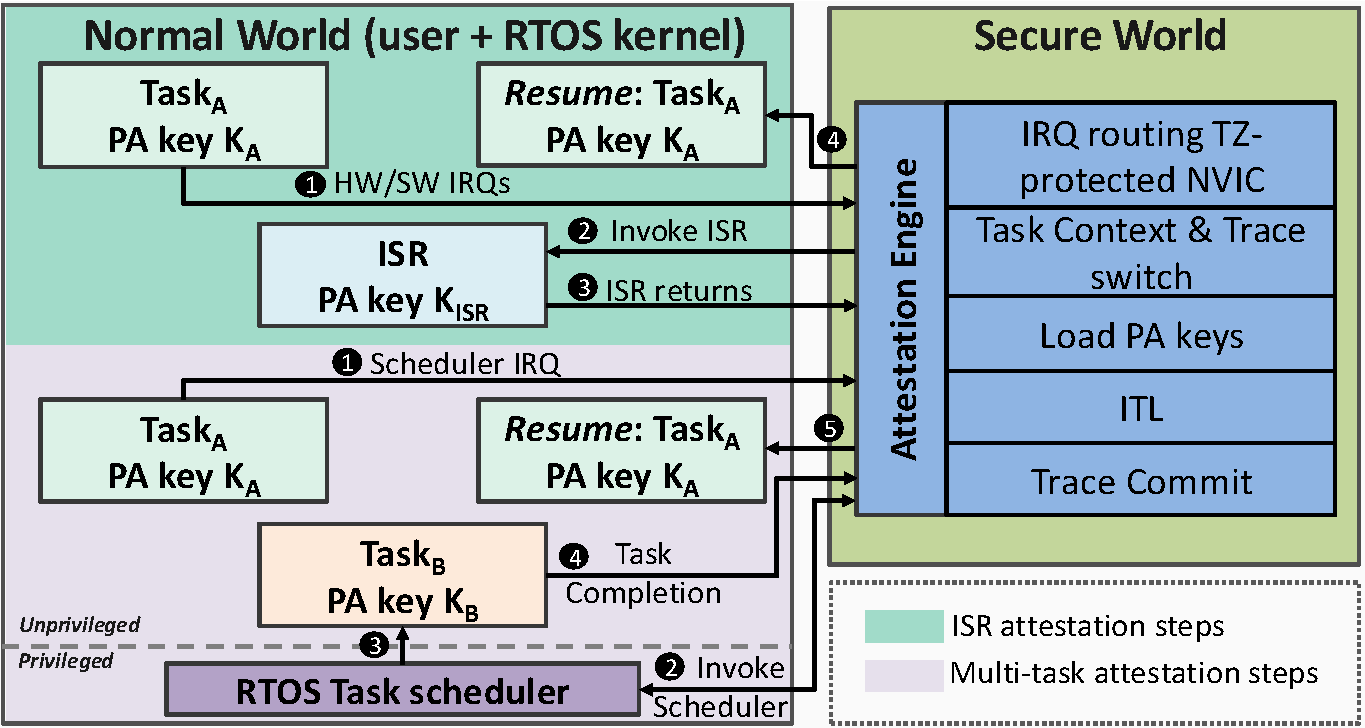
\includegraphics[width=0.46\textwidth]{figs/thrust2.2-rtos-attestation.pdf}
	\caption{Attestation framework for multitask and asynchronous-interrupt handling.}
	\label{fig:thurst22}
	\vspace{-10pt}
\end{wrapfigure}

A central challenge is to protect multiple concurrent measurement states and key bindings, i.e., one per task and ISR, without introducing excessive trusted-world transitions, memory overhead, or replay opportunities across context switches.

Based on the \enola attestation engine~\cite{armanuzzaman2026enola} and its Task~2.1 extension, we will develop a framework that addresses \enola's limitations of interrupt and multitask support, reusing the compiler instrumentation and PA-based measurement strategy described above for each individual execution context.
We will generalize this by assigning each task and ISR its own control-flow representation and per-context occurrence trace, recorded in the MPU-protected, store-hardened region from Task~2.1 rather than through a TrustZone call on every branch.
The interrupt controller and vector table are configured such that interrupts are routed to a transition handler before control reaches the scheduler or the ISR itself (Figure~\ref{fig:thurst22}).
This handler saves the currently active task's execution state and measurement context to the protected region, identifies the interrupt source and the next runnable context.
Because a task's PA key must stay confidential rather than merely tamper-evident -- a guarantee store hardening alone does not provide; thus key switching still crosses into TrustZone.
Before restoring the next task's CPU state, the scheduler triggers a secure call that loads the corresponding key or key slot from a protected task-to-key mapping and binds it to the restored task identity.
This cryptographic binding of each suspended context to its execution identity, key slot, and transition history ensures a compromised task or ISR cannot substitute, or reuse another context's measurement state.
As a result, TrustZone's involvement is confined to per context switch, while evidence for forward branches continues to accumulate in the store-hardened MPU region.
%This confines TrustZone involvement to one call per context switch rather than one per branch, while per-context trace and transition evidence continue to accumulate in the store-hardened region until finalized.
The next task's saved context is restored only after this secure binding has been validated, and the transition is recorded as authenticated evidence for the verifier.

Similarly, for asynchronous interrupt handling, the evidence binds the interrupted task, interrupt source, selected ISR, ISR execution measurement, and authenticated return.
%For execution, the evidence binds task identities, scheduler-mediated transitions, and the corresponding suspend and resume operations.
The same Secure-world call that switches keys also produces a \emph{Trace Commit}: a tag computed over the per-context measurement state while that context's key is exclusively resident, rather than in the exploitable Normal world, tying control-flow evidence to the correct task identity and preventing stale measurement reuse.
Nested interrupts and preemptive scheduling extend this to an authenticated hierarchy of simultaneously suspended contexts.

\begin{comment}
% --- Verifier-side hierarchical execution model, cut to keep Task 2.2
% prover-side, consistent with Task 2.1 -- kept here for reference. ---
At the verifier, we will develop a hierarchical execution model that combines task-specific, ISR-specific, and scheduler control-flow graphs with an authenticated transition graph describing asynchronous and scheduling events.
The verifier will check both \emph{intra-context execution}, determining whether each task or ISR followed an authorized control-flow path, and \emph{inter-context execution}, determining whether interrupt delivery, scheduler decisions, task preemption, context switches, and returns occurred through authorized transitions.
This will enable the verifier to establish not only that individual applications remained protected, but also that the overall interrupt-driven and multitasking execution of the embedded system remained consistent with its expected runtime behavior.
\end{comment}



\textbf{Preliminary Results.}
We implemented and evaluated \enola on the ARM Versatile Express V2M-MPS3 prototyping board configured as a Cortex-M85 microcontroller running at 25 MHz with the AN555 FPGA image and BSP v1.3.0~\cite{ARMMPS3}.
Our software evaluation used the LLVM 16.0.0 ARM embedded toolchain and included a syringe-pump application, the Embench benchmark suite, and the wolfSSL cryptographic library, with multiple compiler optimization levels.
Across Embench, \enola reduced the average attestation data from 21,009 bytes with Blast~\cite{yadav2023whole} to \textbf{397 bytes} under O2 and \textbf{224 bytes} under Oz, corresponding to a reduction of at least \textbf{52$\times$} and demonstrating that the transmitted evidence is linear to program basic blocks rather than execution length.
These results establish the compact, linear-space evidence and hardware-assisted measurement that both tasks build on: Task~2.1 reduces \enola's remaining TrustZone context-switch overhead, and Task~2.2 extends it to interrupt-driven and multitasking execution.

% !TEX root = main.tex
\subsection{Thrust 3: Evidence-Guided Trust Containment and Recovery.}
\label{sb:t3}

\textbf{Problem Statement.}
Most of an embedded device's security-critical and functional logic runs not in the Secure world but as a single, monolithic \emph{Normal-world} RTOS application -- protocol stacks, drivers, RTOS scheduling, and control logic sharing one privilege level and one flat address space. Compartmentalization reduces the blast radius of a compromise here by restricting each component to only the code, data, and peripherals it requires~\cite{clements2018aces,kim2018securing,khan2023ec}, but on resource-constrained MCUs this least-privilege goal is at odds with the hardware available to enforce it: the MPU supports only a small, fixed number of regions, forcing coarse compartments or costly per-transition reconfiguration, and that reconfiguration can itself violate real-time deadlines. Beyond this hardware mismatch, spatial isolation and control-flow protection are rarely composed safely, and correctness under nested, preempting interrupts and DMA-capable peripherals is largely unanalyzed. Even where isolation and control-flow protection both hold, the data that legitimately crosses a compartment boundary remains unconstrained: existing systems restrict \emph{how} compartments may communicate but not \emph{what} they may do with the state they exchange, leaving a confused-deputy gap that a compromised compartment can exploit without violating control-flow policy.
Finally, when a violation is detected, existing systems respond only locally and expose no evidence to a remote verifier, so a contained fault is remotely indistinguishable from a propagated compromise.

This thrust therefore asks the following fundamental question: \textbf{\textit{How can a resource-constrained MCU's Normal-world RTOS application be compartmentalized so that both control flow and the data crossing compartment boundaries are authenticated under real-time and interrupt constraints, and so that a violation produces evidence a remote verifier can use to contain and selectively recover the affected compartment?}} Addressing this question requires new compiler-driven partitioning algorithms that jointly reason about MPU region constraints, real-time budgets, and DMA-capable peripherals; authenticated data-flow policies; interrupt-safe transition mechanisms whose correctness can be formally verified; and evidence-guided recovery protocols that connect to the runtime attestation developed in Thrust~2.

\textbf{Related Work.}
Prior MCU compartmentalization systems partition Normal-world RTOS applications via program-dependence-graph analysis, but none jointly addresses real-time cost, interrupt safety, and data-flow integrity. ACES~\cite{clements2018aces} and EC~\cite{khan2023ec} rely on static dependence analysis, but MPU reconfiguration costs tens of percent of runtime and neither analyzes nested-interrupt correctness; EC further keeps compartments and its own monitor in privileged mode rather than dropping to unprivileged execution, trading CPU-level least privilege for lower porting effort~\cite{khan2023ec}. MINION~\cite{kim2018securing} instead uses coarse, whole-thread views to preserve real-time behavior. None constrains data crossing a compartment boundary: ACES retains write access for up to 80\% of store instructions to a shared variable under its most restrictive policy~\cite{clements2018aces}, and EC's shared-type qualifier grants every compartment full read/write access~\cite{khan2023ec}, leaving a confused-deputy gap exploitable without violating control-flow policy~\cite{chen2005non}. D-Box~\cite{mera2022d} narrows this for DMA channels alone, leaving CPU-writable descriptor fields unprotected.
None of these systems exposes evidence for remote containment and recovery~\cite{clements2018aces,kim2018securing,mera2022d,khan2023ec}, a gap Thrust~3 addresses.

\begin{comment}
% --- Original, longer Problem Statement (pre-shortening), kept for reference. ---
\textbf{Problem Statement.}
Embedded system's bulk of a device's firmware wjtb most security-critical logic and functional logic is not hosted on the Secure-world.
The majority of embedded and cyber-physical application code -- protocol stacks, drivers, RTOS scheduling, and control logic -- continues to execute as a single, monolithic \emph{Normal-world} (non-secure) RTOS application that shares one privilege level and one flat address space, and that must be defended in its own right rather than assumed away by the existence of a separate secure domain.
Compartmentalization reduces the blast radius of a compromise in this Normal-world RTOS code by restricting each firmware component to only the code, data, and peripherals it requires, rather than trusting the entire application with the full ambient privilege of the execution environment~\cite{clements2018aces,kim2018securing,khan2023ec}.
On resource-constrained MCUs, however, this least-privilege goal is fundamentally at odds with the hardware available to enforce it.
The Memory Protection Unit (MPU) supports only a small, fixed number of size- and alignment-constrained regions, forcing compilers and runtimes to either merge unrelated code and data into the same region -- weakening isolation -- or to reconfigure the MPU on every cross-compartment transition, which existing systems show can cost tens of percent of runtime even after aggressive optimization~\cite{clements2018aces,khan2023ec}. Real-time and RTOS-based MCUs face an additional constraint: frequent privilege-mode switching to reconfigure protection state can itself violate deadline guarantees, which is why systems such as MINION~\cite{kim2018securing} restrict themselves to coarse, whole-thread memory views rather than fine-grained code compartments in order to preserve real-time behavior.

A second limitation is that spatial isolation and architectural control-flow protection are rarely composed safely. Existing compartmentalization systems either omit control-flow authentication entirely, allowing a compromised compartment to still reuse any gadget reachable within its own code region~\cite{kim2018securing}, or rely on shared runtime/switching code and shared cross-compartment call metadata that enlarge the set of valid branch targets across compartment boundaries~\cite{clements2018aces,khan2023ec}. Because MPU reconfiguration is not atomic with respect to interrupts, an exception or fault can also be delivered while protection state is only partially updated, and even formally verified enforcement mechanisms have had to acknowledge that a compromised RTOS can mask or override the very debug exceptions used to police this transition~\cite{khan2023ec}. None of these systems analyzes correctness under \emph{nested}, preempting interrupts specifically: ACES does not model interrupts at all; MINION extends its memory-view switching to interrupt entry but does not discuss what happens if a higher-priority interrupt preempts a lower-priority one, or preempts the view-switching routine itself; and EC avoids the question for compartment switches by masking ordinary interrupts for the duration of each switch rather than proving switches correct under nesting. Even production RTOS memory protection fares no better here: FreeRTOS-MPU and Zephyr's memory-domain support run interrupt handlers in privileged mode with unrestricted access to all memory, exempting ISRs from protection entirely rather than reasoning about their safe interleaving with compartment transitions. DMA-capable peripherals compound the problem: because DMA controllers operate outside the CPU's MPU-mediated path, most compartmentalization systems ignore DMA-based attacks altogether, and the one system that does address DMA restricts its capability model to a single peripheral class rather than treating all bus masters uniformly~\cite{mera2022d}.

A third limitation is that even where spatial isolation and control-flow authentication are both enforced, the data that legitimately crosses a compartment boundary remains unconstrained and unverified. Existing systems restrict \emph{how} compartments may communicate, but not \emph{what} they may do with the state they exchange. ACES's own evaluation shows that once a global variable is placed in a shared data region, a median of up to 80\% of the store instructions in the application binary retain write access to it even under its most restrictive policy~\cite{clements2018aces}, and EC's \texttt{shared} type qualifier grants a variable full read/write accessibility to every compartment in the system rather than to only the specific compartments and directions an interaction actually requires~\cite{khan2023ec}. Authenticating that a call reached its intended target compartment does not constrain the values carried across that call: a compromised compartment can still supply a well-formed but malicious argument, or overwrite shared state that another, uncompromised compartment later reads, without violating any control-flow policy. For example, an authorization flag staged in a shared region -- such as the PIN-validity flag in ACES's own PinLock case study~\cite{clements2018aces} -- can be set directly by any compartment holding write access to that region, bypassing the credential check it is meant to gate without triggering any control-flow violation; this is precisely the class of non-control-data attack shown to be a realistic threat even when control-flow integrity holds~\cite{chen2005non}. This is also a form of the classical confused-deputy problem, and existing systems largely acknowledge rather than solve it. ACES restricts and validates only the \emph{locations} of compartment transitions, leaving the values that flow through them unchecked~\cite{clements2018aces}; MINION's own discussion identifies shared data between processes as a residual attack surface that a compromised process can exploit to subvert another~\cite{kim2018securing}; and EC explicitly defers both confused-deputy mitigation and data-flow-aware partitioning to future work~\cite{khan2023ec}. D-Box shows that a capability-based access model can narrow this problem for a single class of shared resource -- DMA channels -- by binding each channel to one task rather than granting ambient access~\cite{mera2022d}, but this protection does not extend to the CPU-side shared memory that general-purpose compartments use to communicate, where the confused-deputy gap remains open: a compartment with legitimate permission to queue a transfer can still overwrite another task's in-flight DMA descriptor -- its source, destination, and length fields, which are ordinary CPU-writable shared memory -- to redirect where the transfer writes, an attack outside the scope of D-Box's channel-ownership model. Recent work outside the MCU compartmentalization literature shows that runtime data-flow integrity (DFI) can be made practical for real-time systems by exploiting slack between average execution time and worst-case execution time reservations~\cite{294543}, but this result targets Cortex-A/Linux-capable platforms with hardware (ARM Memory Tagging Extension) and profiling infrastructure unavailable on resource-constrained Cortex-M MCUs, protects a single task's own instrumented code rather than authenticating data flow across separate compartments, and enforces locally without producing evidence a remote verifier can act on.

A fourth and largely unaddressed limitation is that when a violation is detected, existing systems respond only locally -- typically by faulting or halting the offending compartment -- and expose no evidence to a remote verifier about which compartment was compromised, what it attempted to do, or whether the remaining compartments can still be trusted~\cite{clements2018aces,kim2018securing,mera2022d,khan2023ec}. Consequently, an operator has no principled way to distinguish a localized fault that can be contained and recovered from a compromise that has propagated beyond its compartment boundary, and no way to selectively restore and re-establish trust in only the affected component rather than the entire device.

This thrust therefore asks the following fundamental question: \textbf{\textit{How can a resource-constrained MCU's Normal-world, RTOS-managed application be fine-grained and interrupt-safe compartmentalized so that cross-compartment control-flow transitions and the data they carry are authenticated alongside spatial isolation, and so that runtime violations produce evidence that lets a remote verifier localize the violation, contain it to the affected compartment, and selectively recover and re-attest the rest of the system?}} Addressing this question requires new compiler-driven partitioning algorithms that jointly reason about MPU region constraints, real-time budgets, and DMA-capable peripherals; authenticated data-flow policies that constrain what compartments may read and write across a shared boundary; interrupt-safe transition mechanisms whose correctness can be formally verified; and evidence-guided recovery protocols that connect the local isolation enforced here to the runtime attestation developed in Thrust~2.
\end{comment}




\textbf{Task 3.1: Real-Time- and Data-Flow-Aware Compartmentalization with Interrupt-Safe Transitions.}
We will develop a novel compiler-driven partitioning algorithm that assigns application code and data to compartments using a dependence-graph analysis, with two objectives not considered by existing work: MPU region-budget feasibility under a real-time deadline, and directional separation of a shared variable's readers from its writers.
This dependence analysis is the foundation the remaining tasks in this thrust build their enforcement and recovery mechanisms on.
As shown in Figure~\ref{fig:t31}, the partitioner consumes this dependence graph together with each task's worst-case-execution-time (WCET) budget and produces compartments annotated with directional MPU regions.


\begin{wrapfigure}{r}{0.52\textwidth}
	\centering
	%\vspace{-10pt}
	\begin{tikzpicture}[
			font=\tiny,
			box/.style={draw, rounded corners, align=center, minimum height=0.6cm, inner sep=2pt, fill=white},
			state/.style={draw, rounded corners, align=center, minimum height=0.45cm, minimum width=1.6cm, inner sep=1.5pt, fill=white},
			fstate/.style={draw, rounded corners, dashed, align=center, minimum height=0.45cm, minimum width=1.5cm, inner sep=1.5pt, fill=red!6},
			arr/.style={-{Latex[length=1.4mm]}, thick},
			farr/.style={-{Latex[length=1.4mm]}, thick, dashed, red!55!black},
		]
		% ---- Left column: partitioning pipeline ----
		\node[box, fill=green!14, text width=2.3cm] (pdgwcet) {Dependence graph (control-flow, data, peripherals) + WCET budget};
		\node[box, fill=green!24, text width=2.3cm, below=3mm of pdgwcet] (part) {Real-time- \& data-flow-aware partitioner};
		\node[box, fill=green!8, text width=2.3cm, below=3mm of part] (comp) {Compartments $C_1..C_n$: directional MPU regions (R/O~/~R/W)};
		\draw[arr] (pdgwcet) -- (part);
		\draw[arr] (part) -- (comp);

		% ---- Right column: transition monitor FSM, top-aligned with left column ----
		\node[state, fill=green!6, anchor=north west] (idle) at ($(pdgwcet.north east)+(15mm,0)$) {IDLE};
		\node[state, below=4mm of idle] (revoke) {REVOKE $C_i$};
		\node[state, below=6mm of revoke] (grant) {GRANT $C_j$};
		\node[state, fill=green!6, below=4mm of grant] (commit) {COMMIT: run $C_j$};
		\node[fstate, text width=1.5cm, right=6mm of grant] (fault) {FAULT: access $\leq \min(C_i,C_j)$};

		\draw[arr] (idle) -- node[right]{\texttt{SVC}} (revoke);
		\draw[arr] (revoke) -- node[left]{$C_i$ revoked} (grant);
		\draw[arr] (grant) -- node[right]{$C_j$ granted} (commit);
		\draw[farr] ($(revoke)!0.5!(grant)$) -- node[above,sloped]{NMI/HardFault} (fault);
		\node[font=\tiny, below=1mm of commit] (nextnote) {(next \texttt{SVC} $\to$ IDLE)};
		\node[font=\tiny\bfseries, below=1mm of nextnote, text width=3.6cm, align=center] {Transition monitor FSM, e.g.\ $C_i \to C_j$};
	\end{tikzpicture}
	\vspace{-0.3cm}
	\caption{\textit{Task 3.1}: compartments come from a PDG analysis and real-time budgets (left); every transfer, including DMA commits, drives the transition monitor's verified FSM (right), which stays safe by construction under an NMI/HardFault mid-transition.}
	\label{fig:t31}
	\vspace{-10pt}
\end{wrapfigure}

We will make every cross-compartment control transfer pass through a single trusted transition monitor reached only via \texttt{SVC}.
At boot, the monitor is configured to run at the highest priority any compartment can ever request, and that configuration is then locked against modification by any running compartment.
 %only modifiable by the initial trusted boot sequence -- never a running compartment -- can change it afterward.
Compared to EC's~\cite{khan2023ec} approach of masking interrupts at every switch, which enables a compromised RTOS to divert control flow by priority manipulation, our design fixes non-preemptibility at configuration time, making it resistant to such runtime subversion.
A locked highest priority does not, however, shield the monitor from Cortex-M's \texttt{NMI} and \texttt{HardFault} exceptions, which sit above any configurable priority level and cannot be masked.
To this end, we sequence each MPU region update in fail-safe order, revoking the outgoing compartment's permissions before granting the incoming compartment's, so that any protection state an \texttt{NMI} observes mid-transition is never more permissive than either compartment's legitimate access, only potentially less.
We will formally verify this ordering property and the transition monitor's control logic, following the model-checking and proof-assistant approaches.
Because verifying arbitrary nesting depth is a substantially harder target than the interrupt-masked properties, we will first bound the verified depth to the platform's configured \texttt{NVIC} priority levels, extending to unbounded nesting only if the resulting state space remains tractable.
Finally, we will treat DMA transfer requests as cross-domain calls rather than unilateral peripheral writes: a \textit{trusted DMA broker} validates a compartment's requested source, destination, and length against that compartment's own memory boundaries before committing the descriptor to hardware (Figure~\ref{fig:t31}), protecting the CPU-writable descriptor fields ordinary DMA validation leaves exposed.
Because validating every transfer individually would reintroduce the per-transfer cost DMA exists to avoid, we will amortize this cost across repeated, same-shaped transfers by caching a transfer's shape and cheaply re-authorizing subsequent transfers that match it.

\begin{wrapfigure}{r}{0.48\textwidth}
	\centering
	\vspace{-8pt}
	\begin{tikzpicture}[
			font=\tiny,
			box/.style={draw, rounded corners, align=center, minimum height=0.7cm, inner sep=2.5pt, fill=white},
			mech/.style={draw, rounded corners, align=center, minimum height=0.7cm, inner sep=2pt, fill=gray!12},
			dec/.style={draw, diamond, aspect=2.2, align=center, inner sep=0.5pt, fill=blue!6},
			arr/.style={-{Latex[length=1.6mm]}, thick},
		]
		\node[box, fill=blue!10, text width=2.6cm] (edge) {Def-use edge from Task 3.1's dependence graph};
		\node[dec, below=3mm of edge, text width=2.2cm] (amb) {Statically unambiguous?};
		\node[box, fill=blue!16, text width=1.5cm, below left=4mm and -3mm of amb] (static) {Static MPU region: R/O reader, R/W writer};
		\node[mech, text width=1.5cm, below right=4mm and -3mm of amb] (pa) {PA-tagged write: writer ID, def-site, epoch};
		\node[box, fill=blue!8, text width=2.6cm, below=5mm of amb, yshift=-8mm] (check) {Checked at read, or lazily via evidence stream};
		\draw[arr] (edge) -- (amb);
		\draw[arr] (amb) -- node[above,sloped,pos=0.55]{yes} (static);
		\draw[arr] (amb) -- node[above,sloped,pos=0.55]{no} (pa);
		\draw[arr] (pa) -- (check);
	\end{tikzpicture}
	\caption{\textit{Task 3.2}: unambiguous dependencies get a static, directional MPU region for free; ambiguous ones fall back to a PA-tagged write, checked at read or via the evidence stream.}
	\label{fig:t32}
	\vspace{-10pt}
\end{wrapfigure}
\textbf{Task 3.2: Ambiguity-Guided Data-Flow Integrity.}
Task~3.2 targets the data that legitimately crosses a compartment boundary, authenticating which compartment may write a given shared location rather than leaving all shared state uniformly accessible to every compartment with region access.
The central challenge is enforcing this on Cortex-M, which has no hardware memory-tagging support, without paying full-instrumentation cost for locations the compiler can already resolve statically.

We address this challenge by letting Task~3.1's dependence graph decide, for each shared location, whether it can be protected with a static MPU region or needs a runtime check.
Where the graph proves a single compartment is the only possible writer, we enforce that with a directional MPU region: one compartment gets read-write access, every other compartment gets read-only (or no) access, and the hardware enforces this boundary at no added cost.
Where the graph cannot narrow the writer down to one compartment, due to pointer aliasing or interrupt-interleaved updates (Figure~\ref{fig:t32}), we fall back to a lightweight signature built on ARM's PA hardware: each write computes an authenticator over the writer's identity, the write location, and a monotonically increasing epoch, using the \texttt{PACGA} instruction and the same PA keys Thrust~2 uses for control-flow evidence.
A read recomputes this authenticator and compares it against the small set of candidate-writer keys the dependence graph could not rule out; a compromised compartment outside that set cannot forge a matching tag, and the epoch prevents replaying an old one.
This bounds the confused-deputy gap by constraining which compartment may write a given ambiguous location, while spending its cost only where ambiguity cannot be statically resolved, so overhead scales with program ambiguity rather than with the number of shared variables or the volume of execution.
\begin{comment}
% --- Original Task 3.2 text (pre-rewrite), kept for reference. ---
Building on the same ambiguity-driven philosophy we use for control-flow evidence in Task~2.1, we will treat each data dependency Task~3.1's partitioner exposes across a compartment boundary as either statically resolvable or ambiguous, and enforce it accordingly rather than applying one uniform mechanism to all shared state.
As illustrated in Figure~\ref{fig:t32}, where the dependence analysis can prove a shared location has a single reachable writer for a given reader, we enforce that relationship for free using directional (read-only / read-write) MPU permissions, automating -- and pushing below task granularity -- a distinction that production RTOS memory-protection APIs such as FreeRTOS-MPU and Zephyr's memory domains already expose architecturally but require a developer to configure manually, one task at a time.

Where the analysis cannot statically bound the reaching writer -- due to pointer aliasing or interrupt-interleaved updates, the same conditions that force ACES's own over-approximation~\cite{clements2018aces} -- we fall back to a dynamic mechanism only for that specific dependency, and only among the small candidate set of compartments the analysis could not rule out, rather than trusting any code with region access, as ACES, EC, and MINION do today. Because Cortex-M has no hardware memory-tagging support, each such location is paired with a compact shadow-metadata slot: on write, the compartment computes an authenticator over its own compartment identity, the specific def-site, and the current transition epoch using the \texttt{PACGA} generic-authentication instruction and the same Pointer Authentication key infrastructure Thrust~2 already uses for control-flow measurement, and stores it in that slot. A read -- or, to avoid per-access overhead, the evidence report -- recomputes and compares the authenticator against each key in the candidate-writer set; because producing a valid tag requires the corresponding compartment's key, which untrusted code cannot access, a compromised compartment that can overwrite the metadata slot but does not hold that key still cannot forge a tag that verifies. We will enforce the epoch as a monotonically increasing counter checked for freshness on every read, so that a compromised compartment cannot replay a stale-but-genuinely-valid tag captured from an earlier, legitimate write. This bounds, without fully eliminating, the confused-deputy gap identified in the Problem Statement -- it constrains which compartment may successfully write a given ambiguous location, not whether the value that compartment legitimately chooses to write is itself correct -- and it does so without either the blanket instrumentation cost of classical software DFI~\cite{castro2006securing} or the Cortex-A-only hardware assumptions of opportunistic real-time DFI~\cite{294543}. Because this mechanism spends its cost only where the dependence analysis is genuinely uncertain, we expect its overhead to scale with program ambiguity rather than with the number of shared variables or the volume of execution, mirroring the design goal already validated for control-flow evidence in \enola.
\end{comment}

\textbf{Task 3.3: Evidence-Guided Trust Containment and Recovery.}
We will unify the three enforcement points developed above: MPU faults, transition-monitor violations, and data-flow tag mismatches into a single compact evidence report that extends Task~2.1's encoding with a compartment identifier, the faulting program counter, and the last authenticated transition.
On detecting a violation, the runtime will revoke only the faulting compartment's MPU regions and invalidate its entry in the secure task-to-key mapping.
The same evidence report lets the verifier confirm that no \emph{other} compartment accepted a transition or data-flow tag from the faulting compartment after the point of compromise.
This guarantee is scoped to what Tasks~3.1 and~3.2 authenticate, it does not claim the faulting compartment caused no harm before detection .


\begin{comment}
% --- Figure 9 (fig:t33), removed: largely restates the Task 3.3 prose (violation ->
% localized evidence -> contain/verify -> selective recovery) without adding structure
% not already stated as complete sentences in the text. Kept here for reference. ---
\begin{wrapfigure}{r}{0.48\textwidth}
	\centering
	%\vspace{-8pt}
	\begin{tikzpicture}[
			font=\tiny,
			box/.style={draw, rounded corners, align=center, minimum height=0.7cm, inner sep=2.5pt, fill=white},
			mech/.style={draw, rounded corners, align=center, minimum height=0.7cm, inner sep=2pt, fill=gray!12},
			arr/.style={-{Latex[length=1.6mm]}, thick},
		]
		\node[box, fill=violet!10, text width=2.6cm] (viol) {Violation: MPU fault, FSM violation, or PA tag mismatch};
		\node[mech, text width=2.6cm, below=3mm of viol] (evid) {Localized evidence: compartment ID, fault PC, last transition};
		\node[box, fill=violet!16, text width=1.5cm, below left=3mm and 5mm of evid] (contain) {Contain: revoke MPU regions \& keys};
		\node[box, fill=violet!16, text width=1.5cm, below right=2mm and 5mm of evid] (verify) {Verify: no accepted evidence elsewhere};
		\node[box, fill=violet!8, text width=2.6cm, below=4mm of $(contain)!0.5!(verify)$] (recover) {Selective re-attest \& recover via Thrust~1};
		\draw[arr] (viol) -- (evid);
		\draw[arr] (evid) -- (contain);
		\draw[arr] (evid) -- (verify);
		\draw[arr] (contain) -- (recover);
		\draw[arr] (verify) -- (recover);
	\end{tikzpicture}
	\caption{\textit{Task 3.3}: violations from any enforcement point in Tasks 3.1--3.2 are unified into one evidence report driving localized containment and selective, Thrust-1-based re-attestation of only the affected compartment.}
	\label{fig:t33}
	\vspace{-10pt}
\end{wrapfigure}
\end{comment}

We will then recover the affected compartment rather than the whole device: using Thrust~1's domain-construction and attestation mechanisms, we rebuild compartment's trust measurement, re-verify, and re-admit it into the running system, avoiding a full reboot.
The central challenge is minimizing state revocation lists and per-compartment key storage across compartments to prevent replay attacks or reuse a revoked key, while keeping this bookkeeping within real-time budgets.



% ==========================================================
\section{Evaluation Plan.}
% ==========================================================
\arman{Sectoins starting from here should be about 2-2.5 pages}

% ==========================================================
\section{Broader Impacts.}
% ==========================================================

% ==========================================================
\section{Proposed Project Time line.}
% ==========================================================

% ==========================================================
\section{Results from Prior NSF Support.}
% ==========================================================
The PI has not received prior NSF funding with an award period ending within the last five years and holds no current NSF support. Accordingly, there are no Results from Prior NSF Support to report.

\bibliographystyle{plain}
\bibliography{reference}
\end{document}
